Tato kapitola pojednává o obecném popisu heuristických vyhledávacích a optimalizačních algoritmů inspirovaných přírodou. Jmenovitě se jedná o genetické algoritmy, diferenční evoluci, optimalizaci rojem částic a algoritmus umělých včelstev. Na konci je v krátkosti popsán známý kombinatorický problém obchodního cestujícího a jsou popsány redefinice výše zmíněných evolučních algoritmů pro tento problém řešený v diskrétním prostoru s několika omezujícími podmínkami.

%%%%%%%%%%%%%%%%%%%%%%%%%%%%%%%%%%%%%%%%%%%%%%%%%%%%%%%%%%%%%%%%%%%%%%%%%%%%%%%%%%%%%%%%%%%%%%%%%%%%%%%%%%%%%%%%%%%%%%%%

\section{Genetické algoritmy}
Při studiu genetických algoritmů (ang. \emph{Genetic Algorithms} -- zkratka GA) jsem vycházel z prací~\cite{GAoptimisModel, GAstudy, introductionEvo, optimisationOrderPickingGA}. Genetické algoritmy jsou heuristické vyhledávací nebo optimalizační algoritmy inspirované Darwinovským principem evoluce skrze přirozený výběr. Genetický algoritmus však funguje na vysoké úrovni abstrakce evolučních procesů za účelem \uv{evoluce} řešení pro zadané problémy. Snaží se optimalizovat (tedy minimalizovat či maximalizovat) objektivní funkci, a to za pomoci přechodu z jedné sady chromozomů na novou a to za pomoci genetických operátorů. Genetické algoritmy byly vytvořeny Johnem Hollandem v~roce 1970 za účelem nalezení řešení problémů, které byly výpočetně neřešitelné. Po uvedení se dočkaly velké popularity a rychlého vývoje a byly aplikovány k řešení celé řady problému v různých odvětví jako je věda či průmysl. V dnešní době jsou genetické algoritmy stále velmi aktivní a rostoucí oblast výpočetní inteligence, kam patří mimo jiné například také umělé neuronové sítě~\cite{GAoptimisModel}.

Každý genetický algoritmus pracuje nad populací umělých chromozomů (chromozom je také označován jako jedinec populace), kde každý chromozom představuje jedno řešení problému. Chromozom je konečný řetězec (často binární) a má hodnotu \emph{fitness}, což je desetinné číslo, které udává jak dobrý daný chromozom je. Na začátku výpočtu se provádí inicializace populace, kde se pomocí uniformní náhodné funkce vygenerují hodnoty pro každého jednotlivce v populaci. Dále genetický algoritmus provádí selekci a kombinaci jednotlivců, založenou na velikosti jejich hodnoty \emph{fitness} (dle toho zda se jedná o minimalizační či maximalizační problém), za účelem vytvoření nové generace populace, která bude poskytovat lepší řešení daného problému. Tento proces přirozeného výběru je opakován a nové generace jsou vytvářeny až do chvíle, kdy je splněno kritérium pro zastavení (nalezení optimálního řešení nebo dosažení jistého počtu iterací)~\cite{GAoptimisModel}.

\subsection{Struktura genetických algoritmů}
Genetický algoritmus je velmi modulární (skládá se z několika odlišných částí), což umožňuje znovupoužití jednotlivých částí v jiných genetických algoritmech, usnadňující jejich implementaci. Hlavní části genetického algoritmu jsou kódování genů a chromozomů, fitness funkce (objektivní funkce), křížení jedinců (ang. \emph{crossover}), mutace (ang. \emph{mutation}) a~selekce do další generace na základě fitness funkce, jak lze vidět na obrázku \ref{fig:gaWorkflow}. Za pomoci těchto operátorů genetický algoritmus hledá vhodnější řešení pomocí evoluce a to skrze navazující iterace zvané jako generace~\cite{GAoptimisModel, introductionEvo}.

\begin{figure}[t]
    \centering
    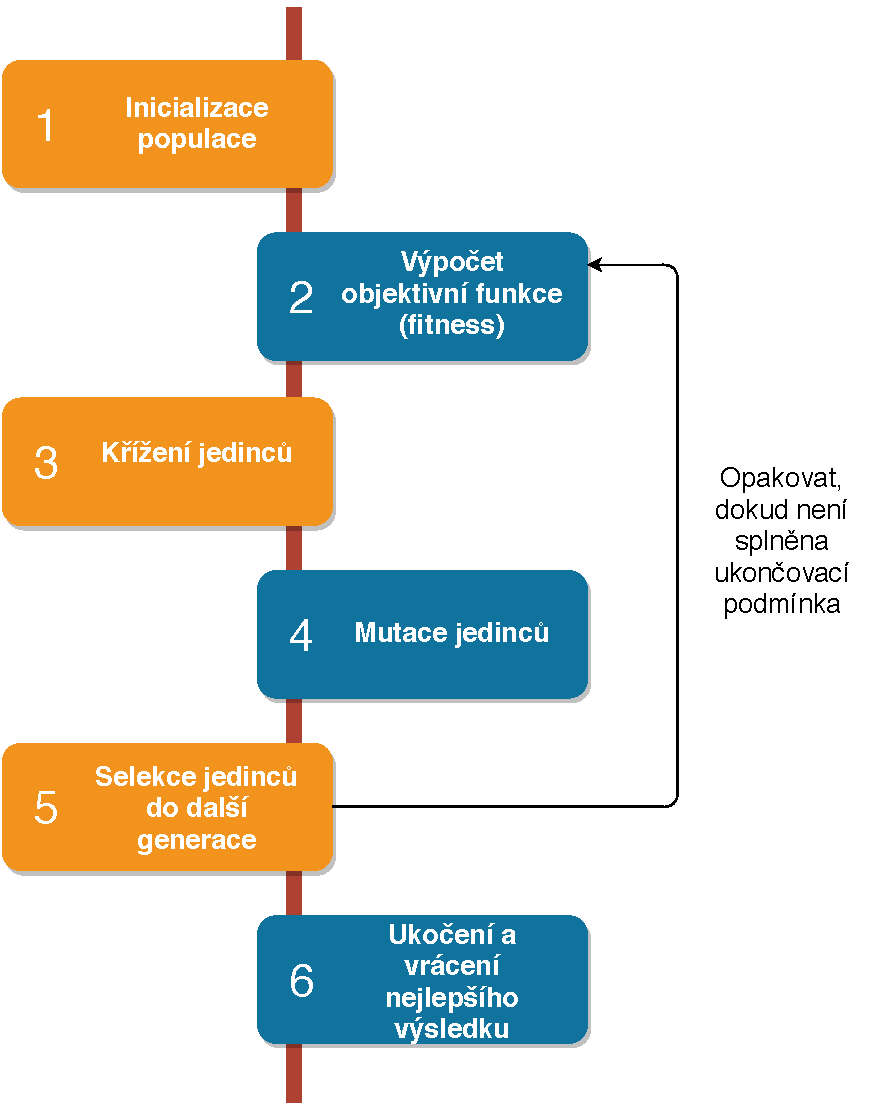
\includegraphics[width=0.50\linewidth]{figures/slap_ea/geneticky_algoritmus.pdf}
    \caption{Princip výpočtu genetického algoritmu. Vytvořeno na základě dat z~\cite{GAoptimisModel}.}
    \label{fig:gaWorkflow}
\end{figure}

\subsubsection{Kódování chromozomů a genů}
Jak již bylo zmíněno, genetický algoritmus modifikuje populaci chromozomů za účelem dosažení lepších jedinců. Chromozomy jsou abstrakcí DNA chromozomů a jsou reprezentovány jako řetězce (často binární), které představují řešení daného problému. Jednotlivé části chromozomu jsou v literatuře nazývány geny a chromozom je tedy řetězec genů určité (konečné) délky. Pozice genu v chromozomu je typicky označována jako \emph{locus}. Hodnota, které gen nabývá se nazývá \uv{\emph{allele}} hodnota. Řešený problém je vždy takzvaně \uv{zakódován} do chromozomů a interpretace této kódované reprezentace se liší problém od problému. Toto je jedna z hlavních výhod genetických algoritmů, a to sice že podobné reprezentace lze použít pro množství různých problémů, umožňující vývoj společných modulů a usnadňující aplikaci genetických algoritmů na nové, zatím neřešené problémy~\cite{GAoptimisModel, introductionEvo}.

\subsubsection{Fitness funkce}
Fitness funkce (objektivní funkce) je výpočetní prostředek, který slouží pro ohodnocení kvality chromozomu vzhledem k jeho schopnosti řešit daný problém, což mimo jiné určuje také pravděpodobnost, s jakou bude daný chromozom vybrán do další generace. Optimální hodnota této funkce se bude lišit v závislosti na řešeném problému, zda se jedná o minimalizační čí maximalizační úlohu. Fitness funkce je opět závislá na řešeném problému a~úzce spojena s kódováním chromozomu, protože značná část interpretace (významu) chromozomu je zakódovaná právě do této fitness funkce~\cite{GAoptimisModel}. 

\subsubsection{Selekce jedinců}
\label{selekceGA}
Selekční operátor slouží pro usměrňování evoluce chromozomů. Do další generace je z populace vybrán jen stanovený počet jedinců, a to, kteří jedinci budou vybráni, závisí zejména na hodnotě fitness jednotlivých prvků (což je diskriminátor kvality jedinců) a z části také na zvoleném selekčním algoritmu. Za účelem zachování diverzity nejsou z populace zpravidla vybráni jen ti nejvhodnější jedinci, ale i jedinci s horší hodnotou fitness (tzn. ne tak dobrá řešení). Jedinci s lepší fitness však můžou být zvýhodňováni, aby nebyl výběr čistě náhodný, ale do další generace se tak dostaly pravděpodobněji ta lepší řešení. Selekce se často provádí s nahrazováním, tzn. lepší chromozomy mohou vybrány vícekrát a dokonce být kombinovány sami se sebou. Zde je přehled několika nejznámějších selekčních metod~\cite{GAoptimisModel, introductionEvo, GAstudy}:

\begin{figure}[t]
    \centering
    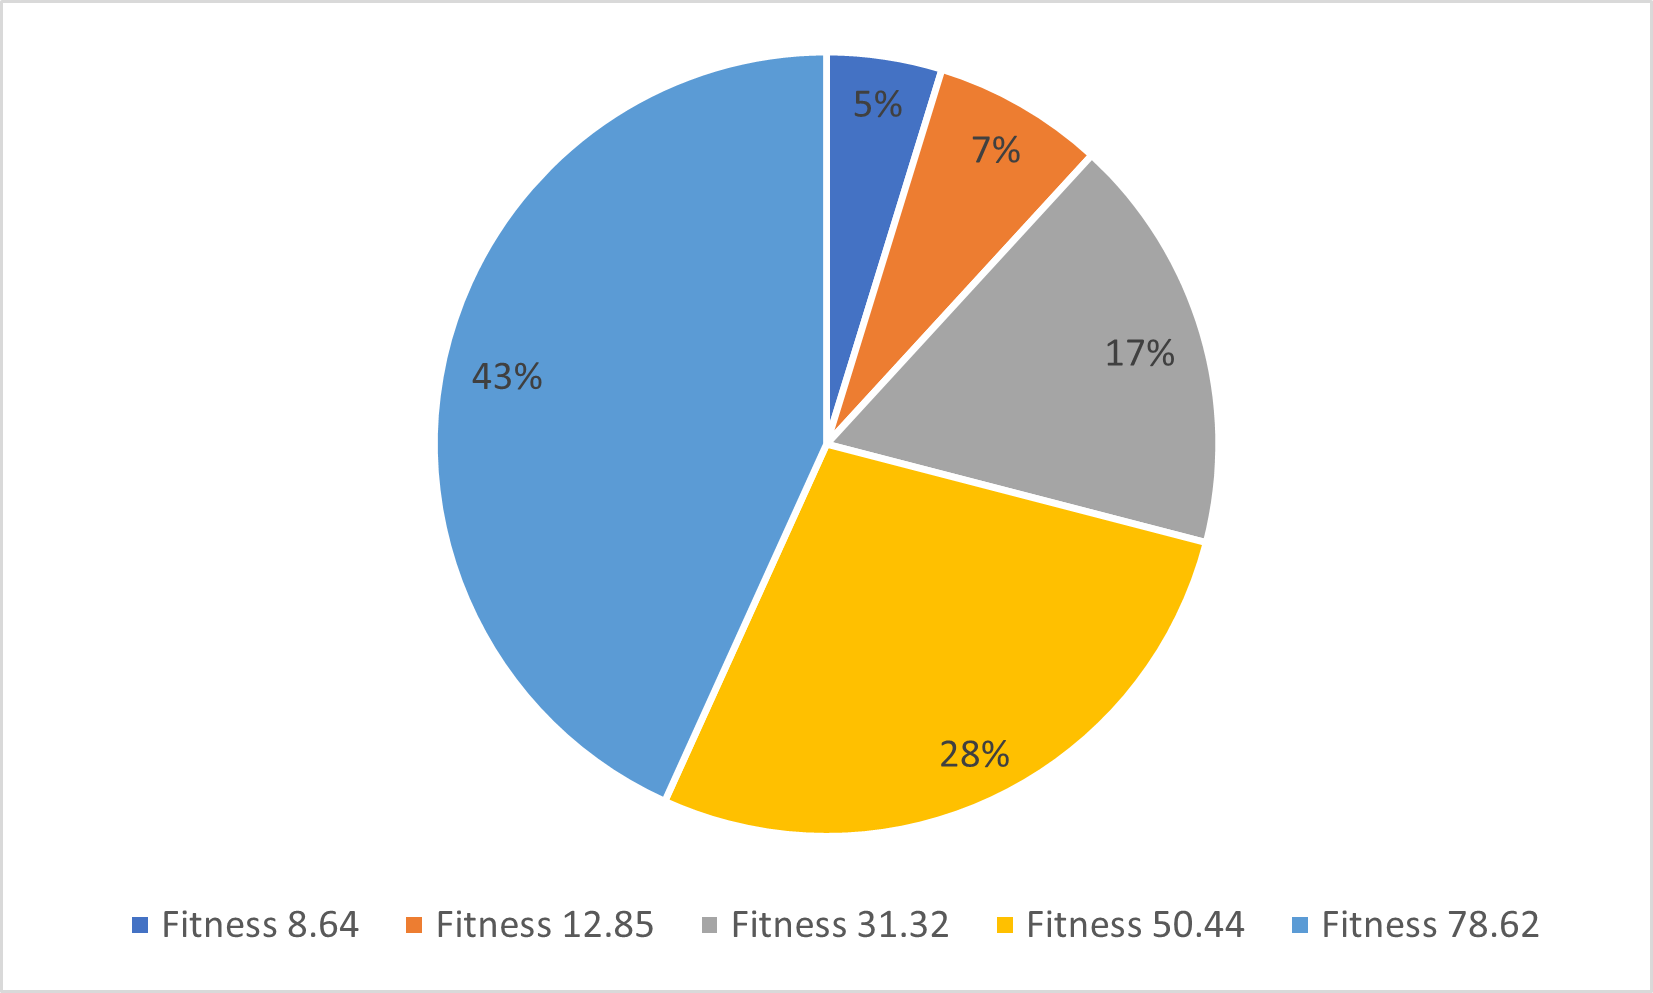
\includegraphics[width=0.9\linewidth]{figures/slap_ea/Roulette.png}
    \caption{Vizualizace příkladu selekce pomocí metody ruleta s pěti jedinci, každý s~různou hodnotou fitness. Největší šanci ($43\%$) na výběr do další generace populace má jedinec s hodnotou fitness $78.62$.}
    \label{fig:roulette}
\end{figure}

\begin{itemize}
    \item \textbf{\emph{Roulette wheel method}} (metoda rulety) -- Je to jedna z nejpoužívanějších metod pro selekci v genetických algoritmech. Zde pravděpodobnost, že bude chromozom vybrán do další generace odpovídá proporčně hodnotě fitness tohoto chromozomu. Tzn. že pravděpodobnost je vypočtena jako hodnota fitness daného chromozomu děleno suma hodnoty fitness všech chromozomů v populaci. V případě, že se jedná o minimalizační problém, by se častěji vybíraly horší řešení, proto je nutné před provedením této metody invertovat hodnoty fitness jednotlivých chromozomů (viz příklad \ref{fig:roulette}).
    \item \textbf{\emph{Rank method}} (metoda \uv{pořadí}) -- Tato metoda v podstatě funguje na stejném principu jako metoda rulety, avšak odstraňuje její největší problém. Metoda rulety má problémy v případě, že hodnota fitness jednotlivých prvků se hodně liší (tzn. pokud jeden chromozom bude zabírat většinu rulety, ostatní nemají téměř žádnou šanci na výběr). Metoda řeší zmíněný problém tak, že seřadí všechny chromozomy na základě jejich fitness, a postupně jim přiřazuje čísla od $1$ po $N$. Tzn. nejvhodnější chromozom bude mít hodnotu $N$, zatímco nejméně vhodný chromozom bude mít hodnotu $1$. Vzhledem k tomu, že tato metoda nezvýhodňuje lepší řešení tak výrazně, má pomalejší konvergenci.
    \item \textbf{\emph{Elittism method}} (\uv{elitní} metoda) -- V době, kdy se vytváří nová generace populace, rovnou překopíruje nejlepší (nebo několik) řešení. To zaručí že algoritmus neztratí nejlepší nalezené řešení, což výrazně zrychluje konvergenci genetického algoritmu.
    \item \textbf{\emph{Tournament metod}} (metoda turnaje) -- Metoda vybere dva (obecně $N$) chromozomů a vybere ten s nejvyšší hodnotou fitness.
    \item \textbf{\emph{Truncation method}} (metoda \uv{zkrácení}) -- Tato metoda vybere z populace náhodně jeden chromozom (s uniformním rozložením pravděpodobnosti).
\end{itemize}


\subsubsection{Křížení jedinců}
\label{krizeniGA}
Vytváření nových jedinců (následníci rodičů) do další generace je v genetických algoritmech prováděno za pomoci sady před-definovaných operátorů. Tyto operátory na vstupu přijímají dva jedince z aktuální generace (rodiče) a produkují na výstup dva nové jedince (potomky). Biologická analogie je kombinování genetického materiálu (DNA), jež se projevuje při reprodukci živočichů. Vzhledem k tomu, že ve většině případů jsou jedinci pro křížení vybírání na základě jejich fitness hodnoty, je pravděpodobné že jejich kombinací vznikne lepší chromozom. Operátor křížení je ve své podstatě nedeterministický, protože se provádí pouze s~určitou pravděpodobností. Také výsledek tohoto operátoru je nedeterministický, protože je založen na stochastické funkci. Operátor křížení má jeden parametr, a to je tzv. \emph{crossover rate}, reprezentující jak často se bude křížení provádět. Při potencionálním křížení se tedy vygeneruje číslo v intervalu $[0,1]$ s uniformním rozložením, pokud je hodnota \emph{crossover rate} vyšší než vygenerované číslo, tak se křížení provede, jinak nikoli. Zde je přehled několika nejznámějších operátorů křížení~\cite{GAoptimisModel, GAstudy}:

\begin{itemize}
    \item \textbf{\emph{One-point crossover}} (operátor křížení jednoho bodu) -- S uniformní pravděpodobností se náhodně vybere číslo $k$ z intervalu $1$ až $N$, kde $N$ je délka chromozomu. Poté se vytvoří potomci takto: První potomek obsahuje řetězec genů $0$ až $k$ z prvního rodiče a zbytek z druhého rodiče. Druhý potomek obsahuje řetězec genů $0$ až $k$ z druhého rodiče a zbytek z prvního rodiče.
    \item \textbf{\emph{Two-point crossover}} (operátor křížení dvou bodů) -- Funguje na stejném principu jako předchozí operátor, ale místo jednoho bodu vybírá dva náhodné body. Potomci poté nesestávají z jedné části z jednoho rodiče a z jedné části z druhého rodiče, nýbrž ze dvou částí z jednoho rodiče a jedné (prostřední) části z druhého rodiče. Tento operátor lze obecně použít na $N$ bodů (\emph{N-point crossover}).
    \item \textbf{\emph{Uniform crossover}} (uniformní operátor křížení) -- Vytváří potomky tak, že prochází rodiče a na každé pozici uniformě vybírá rodiče, ze kterého se použije hodnota allele.
\end{itemize}


\subsubsection{Mutace jedinců}
\label{mutaceGA}
Oproti operátoru křížení, který na základě dvou rodičů vytváří dva potomky, operátor mutace upravuje pouze jednoho jedince. Tyto změny jsou typicky malé, jsou prováděny náhodně a jsou typicky prováděny až po procesu křížení jedinců. Podobně jako u křížení, je i zde definován operátor udávající pravděpodobnost, s jakou bude jedinec mutován (ang. \emph{mutation rate}). Tento operátor funguje stejně jako operátor uvedený u křížení jedinců. Dále je ale definována pravděpodobnost mutace jednotlivých genů. Pravděpodobnost mutace bývá však relativně malá, obzvláště ve srovnání s pravděpodobností křížení. Lze provést například pomocí invertování bitů v binárním řetězci~\cite{GAoptimisModel, GAstudy}.


\subsubsection{Proces evoluce}
Jak již bylo zmíněno, na počátku evoluce je celá populace (všichni jedinci) náhodně inicializovaná. Následně je vyhodnocena fitness funkce pro každý chromozom. Následně se pomocí genetických operátorů vytváří nová generace následníků. Tento proces se skládá z~několika částí, které jsou detailněji popsány výše. První je proveden proces výběru jedinců pro mutování. Takto vybraní jedinci jsou kříženi mezi sebou. Z tohoto procesu vznikne stejný počet potomků, jako do něj vstupuje rodičů a následně jsou někteří z jedinců mutováni. Tito jedinci vstupují do další iterace jako nová generace. Takovýto proces vytváření nových generací je opakován až do doby, kde je buďto splněna podmínka optimalizace/hledání (např. splnění všech podmínek), nebo je dosažen maximální počet generací. Existuje množství různých schémat, jak může genetický algoritmus fungovat. Zde je příklad několika nejběžnějších~\cite{GAoptimisModel, introductionEvo}:

\begin{itemize}
    \item \textbf{Úplné nahrazení} -- V tomto schématu jsou po každé iteraci nahrazeni pomocí genetických operátorů všichni jedinci svými následníky.
    \item \textbf{Ustálené schéma} -- Nová generace je vytvořena generováním jednoho nového následníka každou generaci, který nahrazuje nejméně vhodného jedince předchozí populace.
    \item \textbf{Nahrazení s elitní částí} (nejrozšířenější použití) -- Téměř úplné nahrazení jedinců do další generace (skrze genetické operátory), ale jeden nebo dva jedinci (s nejlepší hodnotou fitness) jsou přesunuti beze změny. Toto schéma zaručuje, že nebudou ztraceny doposud nejlepší výsledky skrze nedeterministický (náhodný) výběr.
\end{itemize}

\begin{table}[htp]
\centering
\caption{Shrnutí genetických algoritmů. Převzato z~\cite{introductionEvo}.}
\label{tab:GA}
\begin{tabular}{|l|l|}
\hline
Reprezentace & Různé druhy, např. bitové řetězce \\ \hline
Křížení & Různé druhy, např. jednobodové křížení \\ \hline
Mutace & Různé druhy, např. inverze bitů \\ \hline
Selekce rodičů & V závislosti na fitness (např. metoda rulety) \\ \hline
Selekce následníků & Generační (následník nahrazuje rodiče) \\ \hline
\end{tabular}
\end{table}


%%%%%%%%%%%%%%%%%%%%%%%%%%%%%%%%%%%%%%%%%%%%%%%%%%%%%%%%%%%%%%%%%%%%%%%%%%%%%%%%%%%%%%%%%%%%%%%%%%%%%%%%%%%%%%%%%%%%%%%%

\section{Diferenční evoluce}
Při studiu diferenční evoluce (ang. \emph{Differential Evolution} -- zkratka DE) jsem vycházel z~\cite{DE_GA_TSP, introductionEvo}. Diferenční evoluce v teorii vychází z genetického algoritmu. Je založena na populaci jedinců a umožňuje provádět tři typy operací s jedinci, a sice: křížení, mutaci a selekci do další generace. Tato metoda je používána k optimalizaci nelineárních funkcí ve spojitém prostoru a pracuje tedy s reálnými čísly. Populace je tvořena jedinci (kandidátní řešení), reprezentovanými vektory reálných čísel $\bar{x} \in \mathbb{R}^n$, v diferenční evoluci také nazývaných jako cílové vektory. Populace je na začátku náhodně inicializována, je vypočtena hodnota fitness pro každého jedince a poté je prováděna optimalizace. Odlišujícím faktorem je že pořadí jedinců v populaci nezávisí na jejich hodnotě fitness a odklonění od použití klasických operátorů evolučních algoritmů~\cite{DE_GA_TSP, introductionEvo}.

\subsubsection{Mutace}
Algoritmus používá tzv. diferenční mutaci, kde nové kandidátní řešení $\bar{v}'$ je získáno přičtením vektoru váženého rozdílu dvou náhodně vybraných jedinců populace:

\begin{align}
    \label{eq:DE1}
    \bar{v}' = \bar{v} + F (\bar{a} - \bar{b}),
\end{align}
kde $F$ reprezentuje faktor škálování, což je reálné číslo, které slouží pro kontrolu rychlosti evoluce. Hodnoty $\bar{a}$ a $\bar{b}$ jsou již zmínění dva náhodně vybraní jedinci populace. Dalším operátorem je operátor křížení, který slouží ke zvýšení diverzity populace~\cite{introductionEvo}.

\subsubsection{Křížení}
V diferenční evoluci se používá uniformní křížení s parametrem $C_r \in \interval[{0,1}]$, který udává pravděpodobnost, s jakou bude (pro jakoukoli pozici v aktuálním rodiči) hodnota \emph{allele} rodiče zahrnuta do potomka, oproti křížení v genetických algoritmech, kde pravděpodobnost udává zda budou daní rodiče vůbec kříženi, či nikoli. Nový cílový vektor $\bar{x}'$ je získán křížením následovně:

\begin{align}
    \label{eq:DE2}
    \bar{x}_k' = \begin{cases}
               \bar{v}_k, & \text{pokud } (U \leq C_r) \lor (j = k) \\
               \bar{x}_k, & \text{jinak}.
               \end{cases}.
\end{align}
Hodnota $U \in \interval[{0,1}]$ označuje náhodně vygenerované reálné číslo. Hodnota $j$ je parametr, který zaručuje, že se potomek bude lišit alespoň jedním \emph{allele} a nakonec hodnota $k$ slouží pro iterování skrze jednotlivé hodnoty \emph{allele}~\cite{DE_GA_TSP}.

\subsubsection{Selekce}
Selekce porovnává fitness nového cílového vektoru (mutovaného a kříženého) s původním. Do další generace je vybrán ten vektor, který má lepší hodnotu fitness:

\begin{align}
    \label{eq:DE3}
    \bar{x} \leftarrow \bar{x}', \text{ pokud } f(\bar{x}') \geq f(\bar{x}),
\end{align}
kde $f$ představuje objektivní funkci pro maximalizační optimalizační problém~\cite{DE_GA_TSP}.

Diferenční evoluce má spoustu variací, např. se liší způsoby jak lze vybírat rodiče. V~literatuře se používá zavedená notace \texttt{DE/x/y/z}, kde \emph{x} reprezentuje výběr rodiče (např. \uv{rand} -- nádhoný rodič, \uv{best} -- nejlepší rodič), \emph{y} je počet diferenčních vektorů a \emph{z} značí použité schéma křížení (např. \uv{bin} je uniformní křížení)~\cite{introductionEvo}.



\begin{table}[htp]
\centering
\caption{Shrnutí diferenční evoluce. Převzato z~\cite{introductionEvo}.}
\label{tab:DE}
\begin{tabular}{|l|l|}
\hline
Reprezentace & Vektor reálných čísel \\ \hline
Křížení & Uniformní křížení\\ \hline
Mutace & Diferenční mutace \\ \hline
Selekce rodičů & \texttt{DE/rand/1/bin} -- náhodně, \texttt{DE/best/1/bin} -- nejlepší, ... \\ \hline
Selekce následníků & Deterministické nahrazení (rodič vs. potomek) \\ \hline
\end{tabular}
\end{table}


%%%%%%%%%%%%%%%%%%%%%%%%%%%%%%%%%%%%%%%%%%%%%%%%%%%%%%%%%%%%%%%%%%%%%%%%%%%%%%%%%%%%%%%%%%%%%%%%%%%%%%%%%%%%%%%%%%%%%%%%

\section{Algoritmus umělých včelstev}
Při studiu algoritmu umělých včelstev (ang. \emph{Artificial Bee Colony} -- zkratka ABC) jsem vycházel z~\cite{ABC, ABC_TSP}. Tento algoritmus analogicky odpovídá chování včelího hnízda a tedy používá včelařskou terminologii. V tomto algoritmu se objevují tři druhy umělých včel, a sice: \uv{zaměstnané} (ang. \emph{employed}), \uv{pozorovací} (ang. \emph{onlooker}) a \uv{průzkumné} (ang. \emph{scout}). Zaměstnaná včela navštěvuje zdroje potravy, kdežto pozorující včela vyčkává za účelem výběru zdroje potravy. Průzkumné včely provádí náhodné hledání zdroje potravy v okolí. V tomto algoritmu spadá první polovina včel do kategorie zaměstnaných, kdežto druhá polovina do kategorie pozorujících a každému zdroji potravy připadá právě jedna zaměstnaná včela. Z toho plyne, že počet zdrojů potravy je přesně roven počtu zaměstnaných včel. Průzkumnými včelami se stávají zaměstnané včely, jejichž zdroj potravy je vyčerpán zaměstnanými a pozorujícími včelami. Proces optimalizace je tedy následovný~\cite{ABC}:

\begin{enumerate}
    \item Náhodná inicializace zdrojů potravy.
    \item Umístění zaměstnaných včel na zdroje potravy v okolí.
    \item Umístění pozorujících včel na zdroje potravy v okolí.
    \item Vyslání průzkumných včel za účelem nalezení nových zdrojů potravy.
    \item Pokud není splněna ukončovací podmínka, vrácení na bod 2.
\end{enumerate}

Každá iterace algoritmu sestává ze třech fází: vyslání zaměstnaných včel na zdroje potravy v okolí a~určení množství nektaru na těchto zdrojích, výběr zdrojů potravy pozorujícími včelami po určení množství nektaru jednotlivých zdrojů a určení průzkumných včel a~jejich vyslání na možné zdroje potravy. V tomto algoritmu je kandidátní řešení problému reprezentováno jako zdroj potravy (potažmo zaměstnaná včela) a kvalitu řešení reprezentuje množství nektaru. To znamená, že čím více nektaru na zdroji potravy je, tím lepší toto řešení je. Zaměstnané a pozorující včely stochasticky modifikují zdroje potravy (řešení) a~vyhodnocují množství nektaru~(fitness). Nový zdroj potravy $v_{ij}$ je ze starého zdroje $x_{ij}$ a sousedního zdroje $x_{kj}$ vytvořen následujícím způsobem:
\begin{align}
    \label{eq:ABC1}
    v_{ij} = x_{ij} + \phi_{ij} (x_{ij} - x_{kj}),
\end{align}
kde $k \in {1, 2, ..., BN}$ a $j \in {1, 2, ... D}$ ($BN$ je počet zdrojů potravy a $D$ je dimenze řešeného problému) jsou náhodně vybrané indexy, kde však musí platit: $i \neq k$. Číslo $\phi_{ij} \in \interval[{-1,1}]$ je také generováno náhodně a slouží k určení dalšího zdroje potravy v okolí, což lze při analogii na reálnou včelu chápat jako vizuální porovnávání zdrojů potravy~\cite{ABC, ABC_TSP}.

Každý zdroj potravy si udržuje hodnotu počtu pokusů. Pokud se množství nektaru v~tomto zdroji zvýší (větší fitness hodnota), tento čítač se vynuluje. Pokud je tomu ovšem naopak a množství nektaru je nižší, tento čítač se zvýší o jedna. Pokud čítač dosáhne předem stanovené hodnoty (tzn. zdroj potravy je vyčerpán), stává se z něj průzkumná včela (tzn. zdroj je znovu náhodně inicializován a je určena jeho hodnota fitness)~\cite{ABC}.



\begin{table}[htp]
\centering
\caption{Shrnutí algoritmu umělých včelstev~\cite{ABC}.}
\label{tab:ABC}
\begin{tabular}{|l|l|}
\hline
Reprezentace & Vektor reálných čísel \\ \hline
Křížení & --- \\ \hline
Mutace & Modifikace zdrojů potravy včelami dle rovnice \ref{eq:ABC1} \\ \hline
Selekce rodičů & Náhodně vybrané zdroje potravy s omezujícími podmínkami \\ \hline
Selekce následníků & Náhodná inicializace zdroje potravy po vyčerpání nektaru \\ \hline
\end{tabular}
\end{table}


%%%%%%%%%%%%%%%%%%%%%%%%%%%%%%%%%%%%%%%%%%%%%%%%%%%%%%%%%%%%%%%%%%%%%%%%%%%%%%%%%%%%%%%%%%%%%%%%%%%%%%%%%%%%%%%%%%%%%%%%

\section{Optimalizace rojem částic}
Při studiu optimalizace rojem částic (ang. \emph{Particle Swarm Optimization} -- zkratka PSO) jsem vycházel z~\cite{PSO_GA_TSP, introductionEvo}. Tento algoritmus je inspirovaný sociálním chováním ptačího hejna, zatímco jméno a použitá terminologie odpovídá spíše fyzickým částicím. Podobně jako u~diferenční evoluce, odlišujícím faktorem je odklonění od použití klasických operátorů evolučních algoritmů a pořadí jedinců v populaci nezávisí na jejich hodnotě fitness. Optimalizace rojem částic nepoužívá operátor křížení a mutace je definována jako sčítání vektorů. Celkový přehled lze nalézt v tabulce \ref{tab:PSO}. Každé možné řešení (tzn. každý jedinec populace) $\bar{x} \in \mathbb{R}^{n}$ s sebou nese také vektor \uv{rychlostí} (ang. \emph{velocities}) $\bar{v} \in \mathbb{R}^{n}$. To znamená, že každé řešení je dvojice $\langle \bar{x}, \bar{v} \rangle$. Vektor rychlostí je později použit pro nalezení nového řešení, tzn. vektoru $\bar{x}$. Hlavní myšlenka algoritmu je tedy v tom, že nová dvojice $\langle \bar{x}', \bar{v}' \rangle$ je vytvořena z~aktuální dvojice $\langle \bar{x}, \bar{v} \rangle$, a to tak, že první se vypočte nový vektor rychlostí, a poté je přičten k řešení~\cite{introductionEvo}:

\begin{align}
    \label{eq:PSO1}
    \bar{x}' = \bar{x} + \bar{v}'.
\end{align}

Každé z řešení je tedy reprezentováno jako bod v prostoru s jistou pozicí a rychlostí, kde rychlost je použita pro výpočet následné pozice. Výpočet rychlosti samotné je v podstatě vážený součet třech komponentů, a to aktuální rychlosti a dvou vektorových rozdílů:

\begin{align}
    \label{eq:PSO2}
    \bar{v}_i = w \bar{v}_i + \phi_1 U_1 (\bar{b}_i - \bar{x}_i) + \phi_2 U_2 (\bar{c} - \bar{x}_i),
\end{align}
kde váhy $w$, $\phi_1$ a $\phi_2$ jsou označovány jako (zleva): $inertia$, faktor učení osobní změny a~faktor učení sociální změny. Hodnoty $U_1$ a $U_2$ jsou náhodně vygenerované z uniformního rozložení v intervalu $\interval[{0,1}]$. Index $i$ značí pozici v populaci/roji. Dále hodnota $\bar{b}$ označuje dosavadní nejlepší výsledek jedince populace, zatímco $\bar{c}$ označuje dosavadní nejlepší výsledek celé populace, kde první z hodnot je třeba uchovávat v paměti pro každého jedince zatímco druhou pouze pro celou populaci. Tento mechanizmus tedy vyžaduje aby jedinci byli jednoznačně identifikovatelní a měli tedy identitu, aby bylo možné upravovat jejich vlastní paměť (nejlepší dosavadní výsledek). Každého jedince populace lze tedy považovat jako trojici $\langle \bar{x}, \bar{v}, \bar{b} \rangle$, značící řešení (pozici), aktuální rychlost a dosavadní nejlepší výsledek jedince. Postup výpočtu je tedy následující~\cite{PSO_GA_TSP, introductionEvo}:

\begin{enumerate}
    \item Náhodná inicializace velikosti roje, pozic částic a rychlosti částic.
    \item Výpočet nové rychlosti částice za pomoci rovnice \eqref{eq:PSO2}.
    \item Výpočet nové pozice částice za pomoci rovnice \eqref{eq:PSO1}.
    \item Aktualizace osobních a globálního nejlepšího výsledku.
    \item Pokud není splněna ukončovací podmínka, vrácení na bod 2.
\end{enumerate}

\begin{table}[htp]
\centering
\caption{Shrnutí optimalizace rojem částic. Převzato z~\cite{introductionEvo}.}
\label{tab:PSO}
\begin{tabular}{|l|l|}
\hline
Reprezentace & Vektor reálných čísel \\ \hline
Křížení & --- \\ \hline
Mutace & Přičtení vektoru rychlostí \\ \hline
Selekce rodičů & Deterministická (rodič vytvoří jednoho následníka pomocí mutace) \\ \hline
Selekce následníků & Generační (následník nahrazuje rodiče) \\ \hline
\end{tabular}
\end{table}

%%%%%%%%%%%%%%%%%%%%%%%%%%%%%%%%%%%%%%%%%%%%%%%%%%%%%%%%%%%%%%%%%%%%%%%%%%%%%%%%%%%%%%%%%%%%%%%%%%%%%%%%%%%%%%%%%%%%%%%%

\section{$\mathcal{MAX}\!{-}\!\mathcal{MIN}$ mravenčí systém}
\label{sec:mmas}
Při studiu $\mathcal{MAX}\!{-}\!\mathcal{MIN}$ mravenčího systému (ang. $\mathcal{MAX}\!{-}\!\mathcal{MIN}$ \emph{Ant System} -- zkratka $\mathcal{MM}$AS) jsem vycházel z prací~\cite{naturalEvoAlgs, MMAS}. Tento algoritmus je, jak název napovídá, inspirovaný chováním mravenčích kolonií. Hlavní princip spočívá v nepřímé komunikaci jedinců populace reprezentujících řešení problému, zvaných mravenci. Komunikace je zajištěna analogií chemické substance zvané feromon, která je periodicky upravována jednotlivými mravenci, reprezentující kvalitu řešení. Algoritmus $\mathcal{MM}$AS je odvozen od původního algoritmu mravenčího systému (ang. \emph{Ant System}), jehož cílem je dosažení lepší výkonnosti zejména při hledání řešení komplexnějších úloh.

Jedná se o variantu mravenčího systému, která na začátku výpočtu všechny hrany inicializuje hodnotou maximální hodnotou feromonu, tedy $\tau_{max}$, což umožňuje lepší prozkoumání řešení na začátku algoritmu. Během aktualizace jsou upraveny pouze hrany, které využilo nejlepší řešení a to buď nejlepší řešení v rámci celého výpočtu nebo pouze v rámci aktuální iterace. Hodnota feromonu každé hrany $\tau_{ij}$ při aktualizaci feromonů je spočtena pomocí rovnice:

\begin{align}
    \label{eq:MMAS1}
    \tau_{ij}(t+1) = \rho \tau_{ij}(t) + \Delta \tau_{ij}^{best},
\end{align}

kde $\Delta \tau_{ij}^{best} = 1/f(s^{best})$ a $f(s^{best})$ značí cenu nejlepšího (globálního či iteračního) řešení. Množství feromonu je omezeno následovně: $\tau_{min} \leq \tau_{ij} \leq \tau_{max}$. Toto omezení je zavedeno kvůli relativně vysoké pravděpodobnosti brzké stagnace vyhledávání způsobené značným důrazem na prohledávání založeném zejména na nejlepším řešení, tzn. aby rozdíly mezi množstvím feromonů jednotlivých hran nebyly příliš obrovské. Dále tento algoritmus často obsahuje opakovanou inicializaci feromonů všech hran hodnotou $\tau_{max}$ ve chvíli, kdy je detekována stagnace vyhledávání. Tento krok do procesu vyhledávání zavede dostatečné množství diverzity, aby se předcházelo stagnaci vyhledávání.

Pokud je pro aktualizaci feromonů použito vždy globální nejlepší řešení, hledací proces se může velmi rychle zaseknout v lokálním minimu a limitovat prohledávání lepších řešení, což může vést ke špatným výsledkům. Riziko uváznutí v lokálním minimu je sníženo, pokud se pro aktualizaci používá nejlepší řešení v rámci iterace, protože to se může značně lišiti každou iteraci a tedy lze dosáhnout diverzity a lepšího prohledávání prostoru. Tyto dva přístupy je ovšem možné také kombinovat.

%%%%%%%%%%%%%%%%%%%%%%%%%%%%%%%%%%%%%%%%%%%%%%%%%%%%%%%%%%%%%%%%%%%%%%%%%%%%%%%%%%%%%%%%%%%%%%%%%%%%%%%%%%%%%%%%%%%%%%%%

\section{Redefinice jednotlivých metod pro diskrétní prostor}
\label{section:redefiniceTSP}
Téměř všechny evoluční algoritmy popsané v této kapitole pracují implicitně ve spojitém prostoru -- tzn. počítají s reálnými čísly. Některé problematiky, jako je například problém obchodního cestujícího nebo problém distribuce a alokace produktů do lokací ve skladu pracují v diskrétním prostoru a tedy počítají s celými čísly. Aby bylo možné evoluční algoritmy na tyto problémy aplikovat, je potřeba provést redefinici algoritmu a s tím související redefinici jeho operátorů (mutace, křížení, ...). V této kapitole bude krátce popsán problém obchodního cestujícího a redefinice jednotlivých metod (vyjma mravenčího algoritmu), aby byly schopny řešit tento problém v diskrétním prostoru. V následujících sekcích je typicky popsáno jen nutné minimum pro fungování v diskrétním prostředí a k řešení problému obchodního cestujícího -- velká část z algoritmů zůstává stejná jako u spojitých verzí algoritmů popsaných dříve v kapitole a tedy zde už není popisována. Důvod, proč je zde tato podkapitola je, že problém obchodního cestujícího je v literatuře velmi často řešeným problémem a~má mnoho společného s problémem řešeným v rámci této práce -- problematikou distribuce a alokace produktů do lokací ve skladu, která je v této práci řešena právě pomocí těchto redefinic evolučních algoritmů.

\subsection{Problém obchodního cestujícího}
\label{section:TSP}
Tento problém by se dal popsat následovně: pokud chce obchodní cestující navštívit každé z $m$ měst právě jednou (kde délka cesty z města $i$ do města $j$ je označována jako $c_{ij}$) a následně se vrátit do počátečního města, jaká je nejkratší taková cesta? Problém obchodního cestujícího spadá do třídy NP-úplných problémů. To znamená, že pokud existuje efektivní řešení (takové, že řeší daný problém v polynomiálním čase) problému obchodního cestujícího, pak existuje efektivní řešení pro každý problém z třídy NP-úplných problémů. Pro formulaci tohoto problému se používá graf $G = (V,E)$, kde $V \in {1,2, ... N}$ jsou uzly reprezentující města a $E$ hrany reprezentující cesty mezi nimi. Každá hrana má cenu, která reprezentuje vzdálenost mezi těmito městy, tzn. čím větší cena hrany, tím delší je cesta mezi těmito městy. Pokud se obchodní cestující může dostat z každého města do kteréhokoli jiného města, pak je graf úplný. Okružní výlet se skládá z jisté podmnožiny uzlů a hran, zvaný obecně jako cesta či v teorii grafů jako Hamiltonova kružnice. Výsledkem algoritmů řešící tento problém je tedy sekvence délky počtu měst s nejnižší cenou (nejkratší cestou), kde se žádné z měst neopakuje a každé sousední město musí být dosažitelné skrze jednu hranu~\cite{TSP, ABC_TSP}.


\subsection{Redefinice genetických algoritmů pro diskrétní prostor}
Při studiu jsem vycházel z~\cite{GA_TSP, orderedCrossover}. Řešení problému obchodního cestujícího (individuum z~populace nebo také chromozom) lze chápat jako cestu složenou z pole genů, kde každý gen reprezentuje jedno město. Město lze reprezentovat například pomocí celočíselného identifikátoru města nebo jeho souřadnic ve formě $(x, y)$. Populace, selekce a fitness fungují na stejném principu jako ve spojitém prostoru, není je tedy potřeba předefinovávat. Je však nutné redefinovat operátory křížení a mutace tak, aby neprodukovaly v řešení duplicitní hodnoty.

\paragraph{Ordered crossover} (česky uspořádané křížení) je křížení, které neporušuje omezení problému obchodního cestujícího specifikované v části \ref{section:TSP}. To znamená že po zkřížení dvou rodičů, potomek bude stále validním řešením a tedy bude obsahovat všechna města a žádné z nich se nebude opakovat. Princip je takový, že pro vytvoření potomka se vybere jedna či více částí cesty z prvního z rodičů. Následně jsou doplněny chybějící města z druhého rodiče a to v takovém pořadí, v jakém se nachází v druhém rodiči. Druhý potomek je vytvořen úplně stejným principem, pouze se role rodičů obrací. Příklad aplikace tohoto operátoru je graficky znázorněn na obrázku \ref{fig:orderedCrossover}.

\begin{figure}[t]
    \centering
    \tmpframe{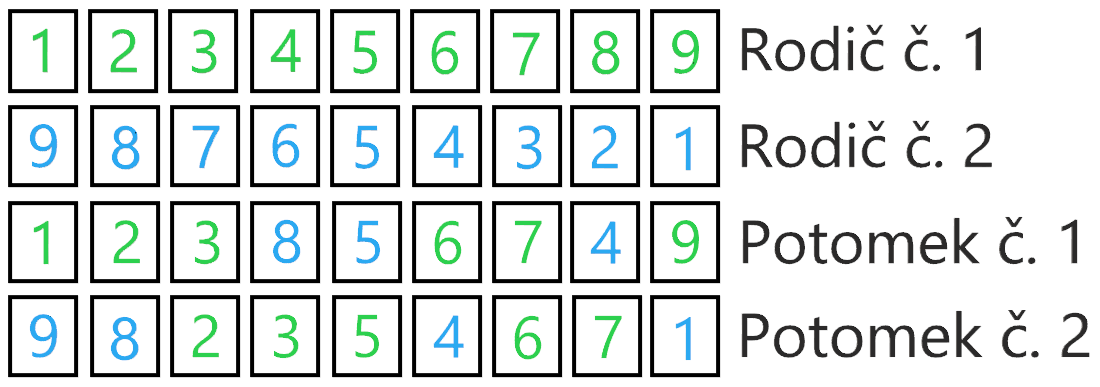
\includegraphics[width=0.7\linewidth]{figures/slap_ea/OrderedCrossover.png}}
    \caption{Graficky znázorněný příklad uspořádaného křížení dvou rodičů~\cite{orderedCrossover}.}
    \label{fig:orderedCrossover}
\end{figure}

\paragraph{Ordered mutation} (česky uspořádaná mutace) je mutace, která obdobně jako uspořádané křížení neporušuje žádné z omezení problému obchodního cestujícího. Funguje na jednoduchém principu přemístění prvku z pozice $A$ na pozici $B$, kde platí, že $A \neq B$. Na tuto mutaci existují různé variance, jako například prohození prvků na indexech $A$ a $B$, či inverze části cesty.


\subsection{Redefinice diferenční evoluce pro diskrétní prostor}
V této sekci je popsána tzv. SBDE -- \emph{step-based differential evolution} (česky volně přeloženo jako \uv{diferenční evoluce založená na krocích}. V této verzi jsou všechny potřebné aritmetické operátory redefinovány následovně~\cite{DE_GA_TSP}:

\paragraph{Element}
Element $(x,y)$ reprezentuje hranu $(x,y)$ mezi městy $x$ a $y$.

\paragraph{Jedinec}
Kandidátní řešení, skládá se z elementů a představuje Hamiltonskou kružnici.

\paragraph{Operátor násobení}
$rand \in \interval[{0,1}] \times \text{element}$ = $rand \in \interval[{0,1}] \times (x,y)$ udává, že element $(x,y)$ bude pro konstrukci nového kandidátního řešení (individua) použit s pravděpodobností $rand$. Při řešení problému obchodního cestujícího výraz $0.3 \times (1,2)$ říká, že hrana $(1,2)$ bude při konstrukci nové cesty navštívena s pravděpodobností $0.3$.

\paragraph{Operátor odečítání}
Pokud $x1$ a $x2$ jsou jedinci populace, potom výraz $x1 - x2 = e \text{ } | \text{ } e \in x1 \land e \not\in x2$, tzn. výsledkem jsou všechny hrany, které jsou v $x1$ a zároveň nejsou v $x2$.

\paragraph{Operátor sčítání}
Pokud se element nachází v obou jedincích, element je použit ve výsledku, a je použita vyšší z pravděpodobností daných elementů se vyskytovat v kandidátním řešení. Pokud se prvek nachází pouze v jednom z dvou řešení, je použit ve výsledku a to se stejnou pravděpodobností.

\paragraph{Výpočet}
\label{binomicalCrossover}
Redefinice aritmetických operátorů pro diskrétní prostor s jistým významem pro řešení problému obchodního cestujícího umožňuje použití binomického křížení, které se vyskytuje v klasické diferenční evoluci. Operátor mutace je třeba trochu upravit, a to následovně:

\begin{align}
    \label{eq:SBDE1}
    \bar{v} = \omega \times x_a + r_{rand} \times (x_b - x_c),
\end{align}

kde $\omega$ a $r_{rand}$ jsou pravděpodobnosti a jsou generovány náhodně pro každý element. V každé iteraci je pro každého jedince náhodně vygenerováno $\alpha \in \interval[{0,1}]$. Každý element v~jedinci, který nemá pravděpodobnost nižší než je hodnota $\alpha$, je umístěn do \uv{sady zbytků}. Z této sady zbytků se poté berou elementy pro konstrukci kandidátního řešení, Hamiltonské kružnice. V případě, že kandidátní řešení ještě není úplné a sada zbytků je již prázdná, je provedeno heuristické vyhledání k doplnění kandidátního řešení (např. hledání nejbližšího souseda). Zbytek je již stejný jako v klasické verzi diferenční evoluce.


\subsection{Redefinice algoritmu umělých včelstev pro diskrétní prostor}
V této sekci je popsáno řešení problému obchodního cestujícího pomocí algoritmu umělých včelstev založeného na \emph{swap sequence} (česky volně přeloženo jako \uv{sekvence výměny}) a~\emph{swap operators} (česky operátory výměny). Ty jsou definovány následovně~\cite{ABC_TSP}:

\paragraph{Operátor výměny}
Pokud $X$ je možné řešení problému, tedy sekvence měst, kterými musí obchodní cestující projít -- Hamiltonská kružnice $X = (x1, x2, ... x_n, x1)$ s množinou měst $V = {1,2, ... N}$, kde $x_i \in V$ a $x_i \neq x_j, \forall i \neq j$, pak je operátor výměny $SO(i,j)$ definován jako výměna měst/uzlů $x_i$ a $x_j$ v možném řešení problému $X$. Symbol $\Diamond$ značí binární operaci výměny a jeho výsledkem obecně je $X' = X \Diamond SO(i,j)$ -- nové možné řešení problému. Příklad: Nechť $X = (x1, x2, x3, x4, x5) = (1, 2, 3, 4, 5)$ je možné řešení problému obchodního cestujícího a $SO(1,4)$ operátor výměny. Poté $X' = X \Diamond SO(1,4) = (1,2,3,4,5) \Diamond SO(1,4) = (4,2,3,1,5)$, a tedy města na indexech $1$ a $4$ jsou prohozena a vzniká nové možné řešení problému $X'$.

\paragraph{Sekvence výměny}
Sekvence dvou a více operátorů výměny se nazývá sekvence výměny. Taková sekvence se značí jako $SS = (SO_1, SO_2, ... SO_n)$, kde $SO_{1,2,...n}$ jsou operátory výměny. Na pořadí jednotlivých operátorů v rámci sekvence záleží a jsou v tomto pořadí aplikovány na možné řešení následovně:

$$
X' = X \Diamond SS = X \Diamond (SO_1, SO_2, ... SO_n) = (...((X \Diamond SO_1) \Diamond SO_2) ... \Diamond SO_n).
$$

Takovéto sekvence výměny lze poté spojovat pomocí operátoru $\oplus$ následovně:

\begin{equation*}
    \begin{split}
        SS' = SS_a \oplus SS_b &= (SO_{a1}, SO_{a2}, ... SO_{an}) \oplus (SO_{b1}, SO_{b2}, ... SO_{bn}) \\
                               &= (SO_{a1}, SO_{a2}, ... SO_{an}, SO_{b1}, SO_{b2}, ... SO_{bn})
    \end{split}
\end{equation*}

Pokud jsou daná možná řešení $X_1$ a $X_2$ a je potřeba najít sekvencí výměny takovou, kterou lze aplikovat na $X_2$ a získat tím $X_1$, tedy rozdíl těchto řešení z pohledu operátorů výměny, lze toho docílit pomocí operátoru $\ominus$.

\paragraph{Výpočet}
Na začátku jsou náhodně inicializovány všechny zdroje potravy, přiřazeny zaměstnaným včelám a vypočtena fitness stejně, jako ve spojité verzi algoritmu. V první fázi zvané \emph{employed}, každá zaměstnaná včela se pokouší zlepšit své řešení náhodným výběrem a aplikací jedné z následujících rovnic:
\begin{align}
    \label{eq:ABC_TSP1}
    Y_i = X_j \Diamond (r \odot (X_i \ominus X_k)),
\end{align}
\begin{align}
    \label{eq:ABC_TSP2}
    Y_i = X_i \Diamond (r \odot (X_j \ominus X_k)),
\end{align}
\begin{align}
    \label{eq:ABC_TSP3}
    Y_i = X_{best} \Diamond (r \odot (X_i \ominus X_k)),
\end{align}
\begin{align}
    \label{eq:ABC_TSP4}
    Y_i = X_i \Diamond (r \odot (X_i \ominus X_{best})),
\end{align}
\begin{align}
    \label{eq:ABC_TSP5}
    Y_i = X_{best} \Diamond (r \odot (X_{best} \ominus X_k)),
\end{align}
\begin{align}
    \label{eq:ABC_TSP6}
    Y_i = X_i \Diamond (r \odot (X_{best} \ominus X_{worst})),
\end{align}
\begin{align}
    \label{eq:ABC_TSP7}
    Y_i = X_i \Diamond (r_1 \odot (X_{best} \ominus X_k) \oplus r_2 \odot (X_k \ominus X_i)),
\end{align}
\begin{align}
    \label{eq:ABC_TSP8}
    Y_i = X_j \Diamond (r \odot (X_{best} \ominus X_i)),
\end{align}
kde $Y_i$ je nové řešení (zdroj potravy) získané z $X_i$ zaměstnanou včelou. $X_j$ a $X_k$ jsou náhodně vybrané zdroje potravy, pro které platí $j \neq k$. Doposud nejlepší řešení je reprezentováno jako $X_{best}$ a podobně, nejhorší řešení jako $X_{worst}$. Výraz $r \odot SS$ udává, že jednotlivé operátory výměny $SO \in SS$ v sekvenci zůstanou s pravděpodobností $r \in \interval[{0,1}]$. To, která z rovnic~\ref{eq:ABC_TSP1}~--~\ref{eq:ABC_TSP8} bude včelou použita, je definováno následovně: každé z rovnic je přiřazen čítač a inicializován na $1$. Pokud je rovnice vybrána, je její čítač zvýšen o $1$. Pravděpodobnost výběru $i$-té rovnice je dána touto rovnicí:

\begin{align}
    \label{eq:ABC_TSP9}
    \rho_i = \frac{v_i}{\sum_{j=1}^{N_{eq}}v_j}, i = 1,2,...N_{eq},
\end{align}

kde $N_{eq}$ značí počet rovnic, a $v_i$ značí rovnici na indexu $i$. Pro každou z rovnic je tedy náhodně vygenerováno $r \in \interval[{0,1}]$ a spočteno $\rho_i$, pokud platí, že $r < \rho_i$, je vybrána rovnice $v_i$ a provedena její aplikace. Poté se znovu vyhodnotí fitness -- tj. množství nektaru a algoritmus se opakuje. Zbytek je již stejný jako v klasické verzi algoritmu.

\subsection{Redefinice optimalizace rojem částic pro diskrétní prostor}
V této sekci je popsán algoritmus pro řešení problému obchodního cestujícího pomocí optimalizace rojem částic (v kombinaci s genetickými algoritmy) využívající heuristické křížení jedinců, jehož algoritmus lze vidět v pseudokódu \ref{alg:diskretniPSO}. Postup výpočtu redefinovaného algoritmu je následující: Na začátku je inicializován roj o velikosti $s$ náhodně. To znamená, že každá částice má náhodnou pozici a pro každou částici se nastaví osobní nejlepší výsledek na aktuální náhodně inicializovanou hodnotu. Následně je pro každou částici vypočtena hodnota fitness pomocí objektivní funkce a je vybráno globální maximum. Pro každou částici je vypočtena nová pozice takto: $x = b^x_p \otimes b_g$, kde $b^x_p$ značí dosavadní osobní maximum prvku $x$, $b_g$ značí dosavadní globální maximum všech částic a operátor $\otimes$ značí heuristické křížení popsané v pseudokódu \ref{alg:diskretniPSO}. Poté je pro každou nově spočtenou částici znovu vyhodnocena objektivní funkce, a pokud je nová hodnota lepší než hodnota osobního nejlepšího výsledku, je osobní nejlepší výsledek přepsán touto novou hodnotou. Po takovémto přepočítání všech částic je znovu vyhodnoceno globální maximum. Takové přepočítávání pozic a znovu vyhodnocování objektivní funkce se opakuje až do doby, kdy je splněna některá z~ukončovacích podmínek~\cite{PSO_GA_TSP}.

\begin{algorithm}[H]
	\caption{Heuristické křížení jedinců~\cite{PSO_GA_TSP}.}
	\label{alg:diskretniPSO}
	\hspace*{\algorithmicindent} \textbf{Vstup:} Dva jedinci $x_1$ a $x_2$\\
    \hspace*{\algorithmicindent} \textbf{Výstup:} Jedinec $x$\\
    \hspace*{\algorithmicindent} \textbf{Kroky:}
	\begin{algorithmic}[1]
	    \State Výběr náhodného města $v$
	    \State Přesun města $v$ na začátek $x_1$ a $x_2$
	    \State Inicializace $x$ pomocí $v$

		\For {$i,j=2,\ldots,n$}
			\If {$x_1[i] \in x \text{ and } x_2[j] \in x$}
			    \State $i = i + 1$
			    \State $j = j + 1$
			\ElsIf {$x_1[i] \in x$}
			    \State Konkatenace $x_2[j] \text{ k } x$
			    \State $j = j + 1$
			\ElsIf {$x_2[j] \in x$}
			    \State Konkatenace $x_1[i] \text{ k } x$
			    \State $i = i + 1$
			\Else
			    \State Nechť $u$ je poslední město v $x$
			    \If {$\text{vzdálenost}(u, x_1[i]) < \text{vzdálenost}(u, x_2[j])$}
			        \State Konkatenace $x_1[i] \text{ k } x$
			        \State $i = i + 1$
			    \Else
			        \State Konkatenace $x_2[j] \text{ k } x$
			        \State $j = j + 1$
			    \EndIf
			\EndIf
		\EndFor
	\end{algorithmic} 
\end{algorithm}

